% Template for ICIP-2015 paper; to be used with:
%          spconf.sty  - ICASSP/ICIP LaTeX style file, and
%          IEEEbib.bst - IEEE bibliography style file.
% --------------------------------------------------------------------------
\documentclass{article}
\usepackage{spconf,amsmath,graphicx}
\usepackage{listings}
\usepackage{float}
\usepackage{pythonhighlight}
\usepackage{comment}
% Example definitions.
% -------------------\def\x{{\mathbf x}}
\def\L{{\cal L}}

% Title.
% ------
\title{Processamento Digital de Imagens - Trabalho 4}
%
% Single address.
% ---------------
\name{Bruna Medeiros da Silva - 16/0048711}
\address{UnB - FGA}
%
% For example:
% ------------
%\address{School\\
%	Department\\
%	Address}
%
% Two addresses (uncomment and modify for two-address case).
% ----------------------------------------------------------
%\twoauthors
%  {A. Author-one, B. Author-two\sthanks{Thanks to XYZ agency for funding.}}
%	{School A-B\\
%	Department A-B\\
%	Address A-B}
%  {C. Author-three, D. Author-four\sthanks{The fourth author performed the work
%	while at ...}}
%	{School C-D\\
%	Department C-D\\
%	Address C-D}
%
\begin{document}
%\ninept
%
\maketitle

%
\section{Questão 1 - Region Labeling Algorithm}
Algoritmos de rotulação de componentes são algoritmos desenvolvidos para detectar a presença de objetos dentro da imagem e identificar suas posições, rotulando-os.

Essa detecção pode ser feita utilizando 3 métodos:

\begin{itemize}
	\item \textbf{\textit{Recursive Tracking}}, que raramente é utilizado;
	\item \textbf{\textit{Parallel Growing}}, que necessita de computação paralela e
	 \item \textbf{\textit{Row-by-Row}}, que faz uso de um algoritmo mais simples e é o mais comumente utilizado.
\end{itemize}

Com isso, a técnica utilizada para o desenvolvimento desse algoritmo, foi pelo método Row-by-Row.

\subsection{Metodologia}
Para chegar ao resultado esperado, a imagem foi percorrida 2 vezes. Para a primeira, onde realiza-se uma primeira rotulação dos componentes, de  foram aplicados os seguintes passos:

\begin{enumerate}
	\item Binarização da imagem, utilizando limiares (\textit{threshold}) de acordo com a necessidade visualizada para cada imagem;
	\item Pré-processamento/Tratamento morfológico da imagem, com o objetivo de preencher buracos;
	\item Percorre-se a imagem de linha em linha, analisando a vizinhança de 8 de cada pixel;
	\item Se o pixel em questão for 1 e vier depois de um zero, será definido como um novo componente, utilizando o menor valor inteiro positivo ainda não utilizado para rotulação;
	\item Se esse mesmo pixel tiver algum vizinho já percorrido com um valor menor que ele, deve-se armazenar o valor mais baixo entre eles, utilizar um dicionário ou algo que relacione os dois identificadores para uma modificação posterior.	
\end{enumerate}

Nesse segundo momento, deve-se percorrer novamente a imagem, linha por linha, para realizar as alterações dos casos de conflito, substituindo sempre os valores mais altos pelos mais baixos. Nessa segunda vez em que percorre-se a imagem, fazesse no intuito de realizar as substituições nos casos de conflito, substituindo sempre o valor mais alto pelo mais baixo dentro da vizinhança do pixel. Para realizar essa operação é utilizada uma condicional dentro dos loops que percorrem as colunas e linhas da imagem, verificando o valor dos pixels e substituindo-os. 

As principais operações morfológicas utilizadas nessa etapa foram as operações de fechamento,  visando cobrir "rastros" de pixels vazios dentro da imagem. 

Nas Figuras \ref{fig: test1} a \ref{fig: test7} te

\begin{figure}[!ht]
	\begin{minipage}[b]{1.0\linewidth}
		\centering
		\centerline{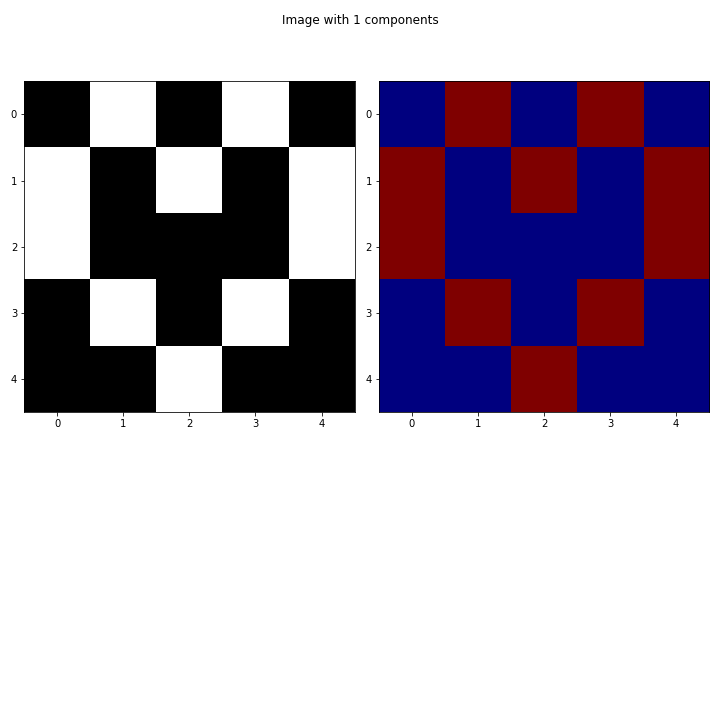
\includegraphics[width=7cm]{Figures/test1.png}}
		\label{fig: test1}
		\vspace{-2.0cm}		
		\centerline{Figura de teste 1 do algoritmo de Rotulação de componentes}\medskip
			
	\end{minipage}

\end{figure}

\begin{figure}[!ht]
	\begin{minipage}[b]{1.0\linewidth}
		\centering
		\centerline{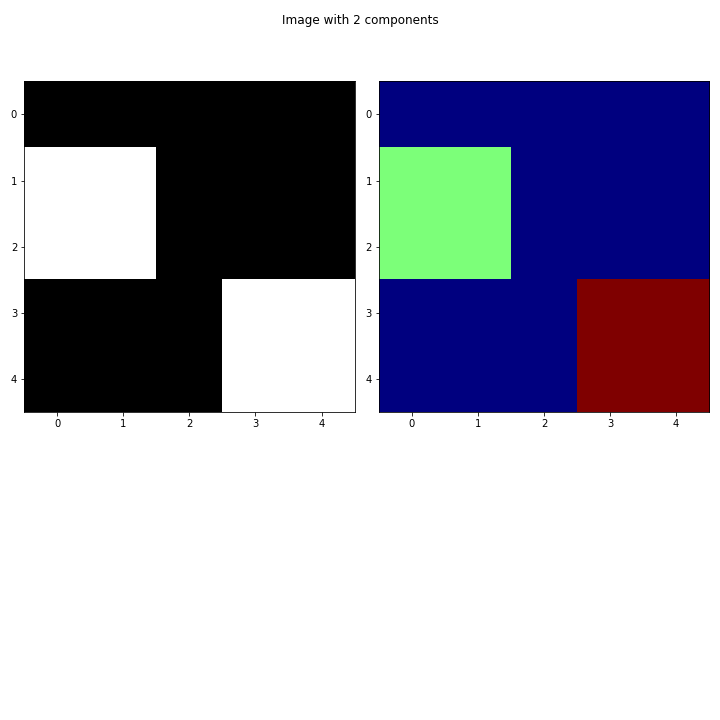
\includegraphics[width=7cm]{Figures/test2.png}}
		\label{fig: test2}
		\vspace{-2.0cm}
		\centerline{Figura de teste 2 do algoritmo de Rotulação de componentes}\medskip
	\end{minipage}	
\end{figure}

\begin{figure}[!ht]
	\begin{minipage}[b]{1.0\linewidth}
		\centering
		\centerline{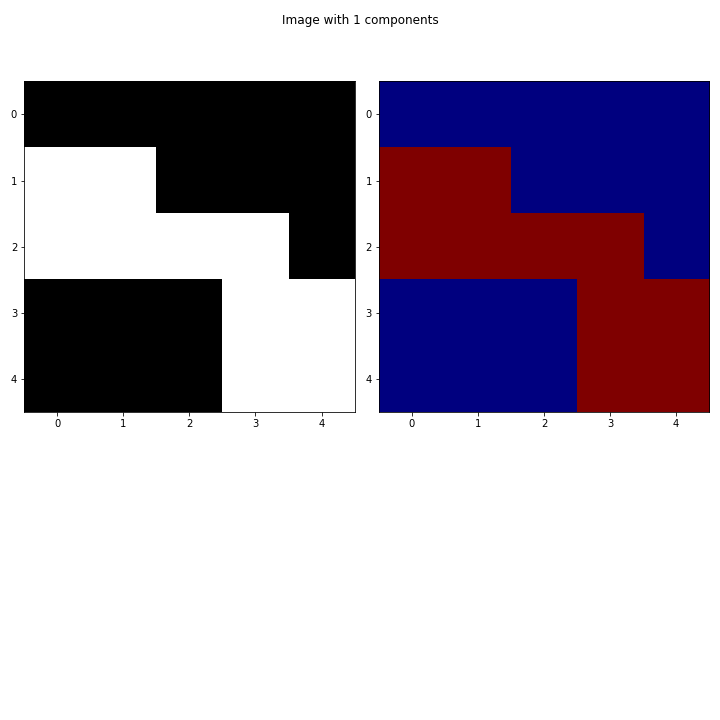
\includegraphics[width=7cm]{Figures/test3.png}}
		\label{fig: test3}
		\vspace{-2.0cm}
		\centerline{Figura de teste 3 do algoritmo de Rotulação de componentes}\medskip	
	\end{minipage}
\end{figure}

\begin{figure}[!ht]
	\begin{minipage}[b]{1.0\linewidth}
		\centering
		\centerline{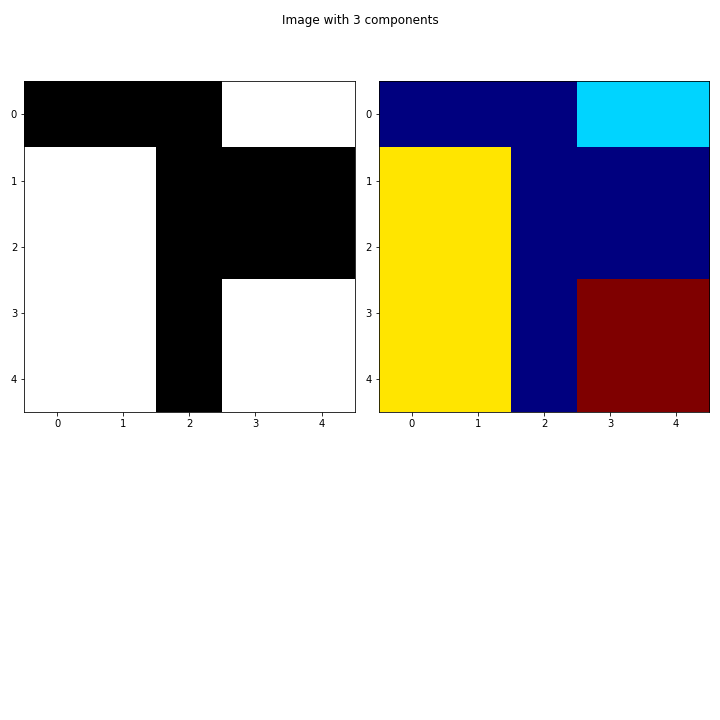
\includegraphics[width=7cm]{Figures/test4.png}}
		\label{fig: test4}	
		\vspace{-2.0cm}
		\centerline{Figura de teste 4 do algoritmo de Rotulação de componentes}\medskip
	\end{minipage}
\end{figure}

\begin{figure}[!ht]
	\begin{minipage}[b]{1.0\linewidth}
		\centering
		\centerline{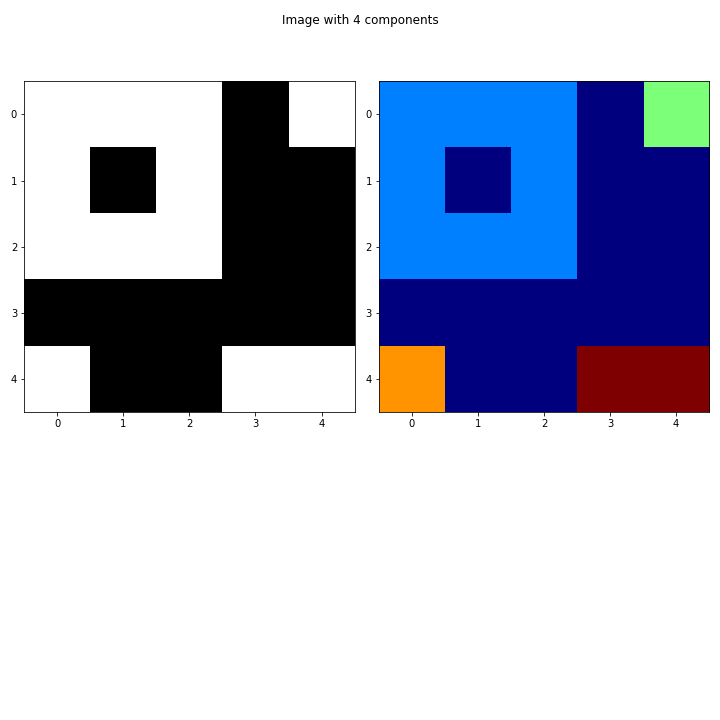
\includegraphics[width=7cm]{Figures/test5.png}}
		\label{fig: test5}
		\vspace{-2.0cm}
		\centerline{Figura de teste 5 do algoritmo de Rotulação de componentes}\medskip	
	\end{minipage}
\end{figure}

\begin{figure}[!ht]
	
	\begin{minipage}[b]{1.0\linewidth}
		\centering
		\centerline{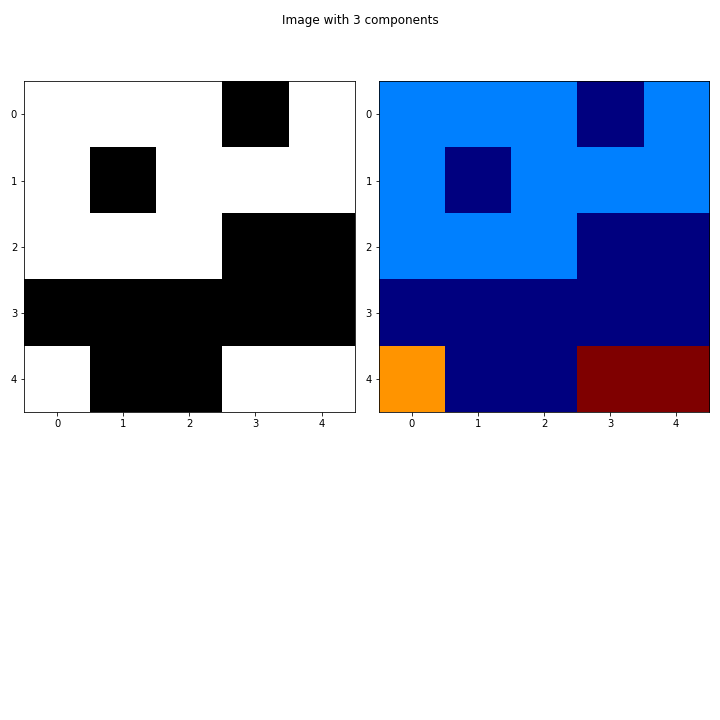
\includegraphics[width=7cm]{Figures/test6.png}}
		\label{fig: test6}
		\vspace{-2.0cm}
		\centerline{Figura de teste 6 do algoritmo de Rotulação de componentes}\medskip	
	\end{minipage}
\end{figure}

\begin{figure}[!ht]
	\begin{minipage}[b]{1.0\linewidth}
		\centering
		\centerline{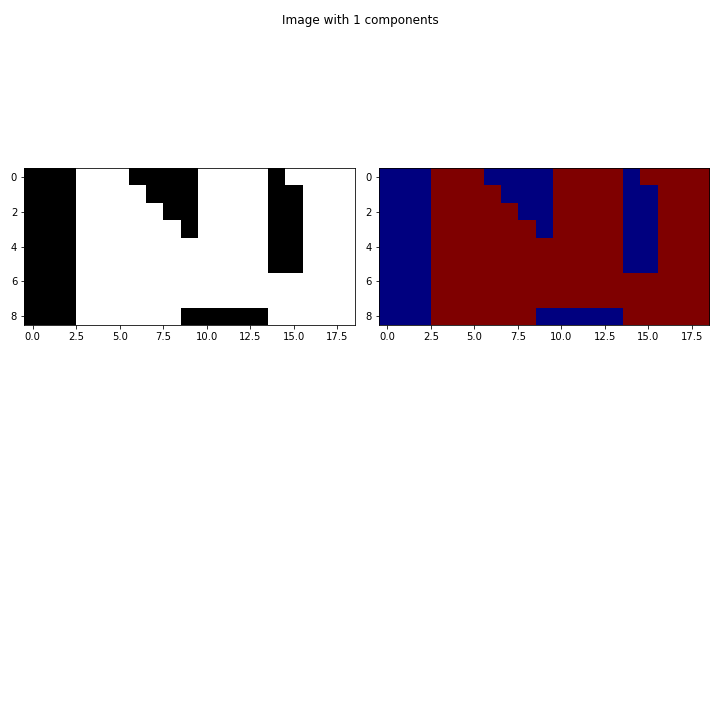
\includegraphics[width=7cm]{Figures/test7.png}}
		\label{fig: test7}
		\vspace{-2.0cm}
		\centerline{Figura de teste 7 do algoritmo de Rotulação de componentes}\medskip	
	\end{minipage}
\end{figure}

Na detecção e separação dos objetos da imagem, visto que cada mancha possui seu próprio número identificador (o valor dos pixels atribuído) , obteve-se os extremos em X e em Y com esse dado valor, gerando uma imagem retangular contendo toda a mancha. 


Para identificar os resultados alcançado foi muito melhor realizando um processo de detecção de bordas (gradiente), invertendo da imagem e aplicando novamente o algoritmo de detecção de componentes sobre o resultado, obtendo uma maior taxa de acertos quando comparado a casos utilizando apenas processamento morfológico de diversos tipos.  Com isso, a quantidade de manchas detectadas passa a ser a quantidade de buracos existentes. 

Para contabilizar a porcentagem do componente composto por buracos, construiu-se um algoritmo que novamente detecta as bordas de cada linha da imagem, considerando os pontos pretos (zeros) nesse intervalo como buracos. Essa quantidade será somada, linha a linha, e divida no final pela quantidade total de pixels, que também é somada a cada iteração. O valor obtido será considerado a porcentagem de buracos dentro de cada mancha.
 	
\subsection{Resultados}
Aplicando os códigos construídos nas imagens entregues pelo professor, buscou-se realizar diversos tipos de tratamento nas imagens. Porém, alguns casos mostraram resultados não tão satifastórios, gerando problemas durante a detecção de manchas e buracos.

\subsubsection{Fig1}
O resultado da aplicação do primeiro código à imagem \textbf{fig1.jpg} pode ser visto na Figura \ref{fig: ccl_fig1}. Já o resultado do código de detecção de buracos se encontra na Figura \ref{fig: hole_fig1}. 

O Código \ref{cod:ccl_fig1} foi o código utilizado para chegar nos resultados descritos para esta imagem. 

\begin{figure}[!ht]
	\begin{minipage}[b]{1.0\linewidth}
		\centering
		\centerline{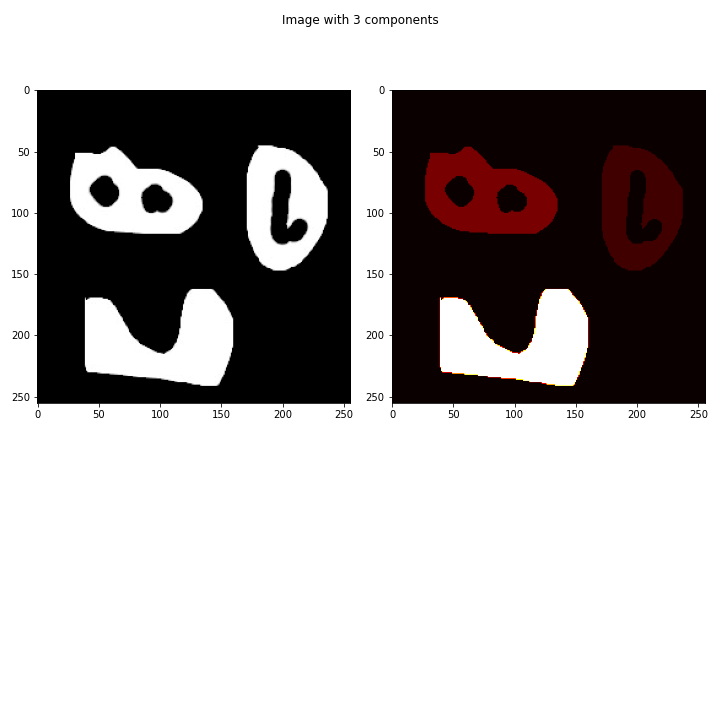
\includegraphics[width=7cm]{Figures/fig1.png}}
		\label{fig: ccl_fig1}
		\vspace{-2.0cm}
		\centerline{Fig1 após passar pelo processo de rotulação de componentes}\medskip	
	\end{minipage}
\end{figure}

\begin{figure}[!ht]
	\begin{minipage}[b]{1.0\linewidth}
		\centering
		\centerline{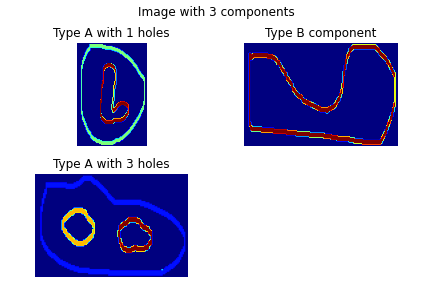
\includegraphics[width=7cm]{Figures/ccl_fig1.png}}
		\label{fig: hole_fig1}
	%	\vspace{-2.0cm}
		\centerline{Fig1 após passar pelo processo de detecção de buracos}\medskip	
	\end{minipage}
\end{figure}


\subsubsection{Fig2}
O resultado da aplicação do primeiro código à imagem \textbf{fig2.jpg} pode ser visto na Figura \ref{fig: ccl_fig2}. Já o resultado do código de detecção de buracos se encontra na Figura \ref{fig: hole_fig2}.

O Código \ref{cod:ccl_fig2} foi o código utilizado para chegar nos resultados descritos para esta imagem. Como pode-se notar, a segunda parte da atividade não foi aplicada a essa figura, especificamente. Isso porque, devido aos problemas na detecção das manchas, a aplicação desse código gera diversos erros. Dessa forma, optou-se por não aplicar estes resultados finais.

\begin{figure}[!ht]
	\begin{minipage}[b]{1.0\linewidth}
		\centering
		\centerline{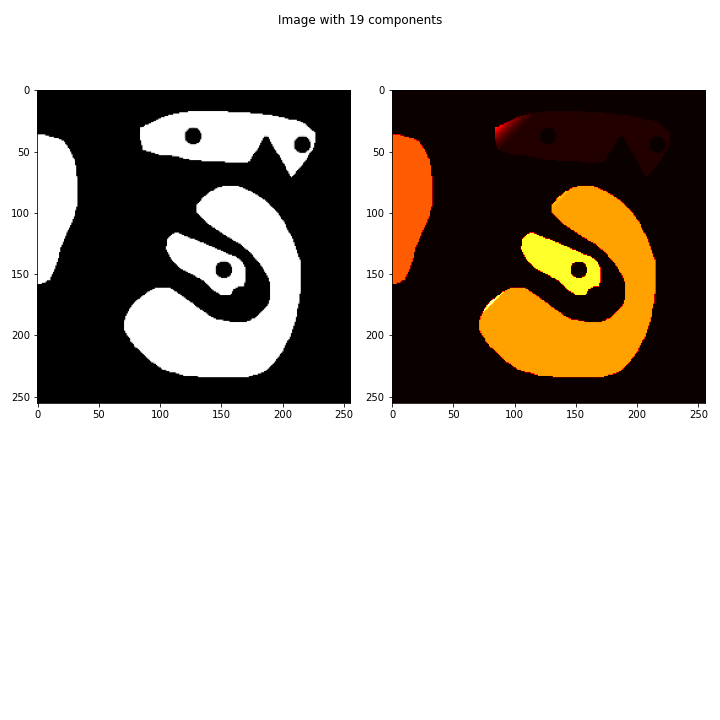
\includegraphics[width=7cm]{Figures/fig2.png}}
		\label{fig: ccl_fig2}
		\vspace{-2.0cm}
		\centerline{Fig2 após passar pelo processo de rotulação de componentes}\medskip	
	\end{minipage}
\end{figure}

\begin{comment}
\begin{figure}[!ht]
	\begin{minipage}[b]{1.0\linewidth}
		\centering
		\centerline{\includegraphics[width=7cm]{Figures/ccl_fig2.png}}
		\label{fig: hole_fig2}
		\vspace{-2.0cm}
		\centerline{Fig1 após passar pelo processo de detecção de buracos}\medskip	
	\end{minipage}
\end{figure}
\end{comment}

\subsubsection{Fig3}
O resultado da aplicação do primeiro código à imagem \textbf{fig3.jpg} pode ser visto na Figura \ref{fig: ccl_fig3}. Já o resultado do código de detecção de buracos se encontra na Figura \ref{fig: hole_fig3}.  

O Código \ref{cod:ccl_fig3} foi o código utilizado para chegar nos resultados descritos para esta imagem.

\begin{figure}[!ht]
	\begin{minipage}[b]{1.0\linewidth}
		\centering
		\centerline{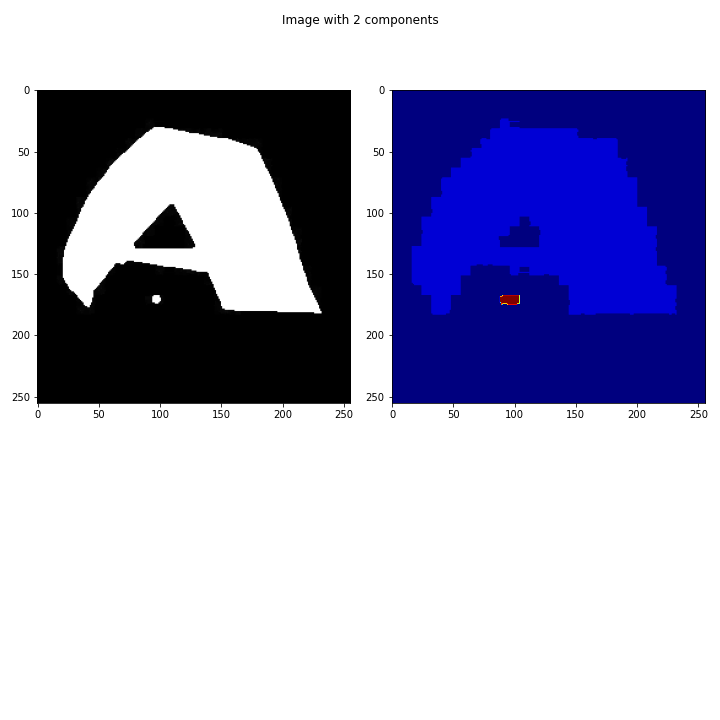
\includegraphics[width=7cm]{Figures/fig3.png}}
		\label{fig: ccl_fig3}
		%\vspace{-2.0cm}
		\centerline{Fig3 após passar pelo processo de rotulação de componentes}\medskip	
	\end{minipage}
\end{figure}

\begin{figure}[!ht]
	\begin{minipage}[b]{1.0\linewidth}
		\centering
		\centerline{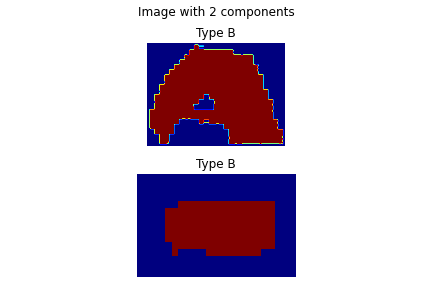
\includegraphics[width=7cm]{Figures/ccl_fig3.png}}
		\label{fig: hole_fig3}
	%	\vspace{-2.0cm}
		\centerline{Fig1 após passar pelo processo de detecção de buracos}\medskip	
	\end{minipage}
\end{figure}

\subsubsection{Fig4}
O resultado da aplicação do primeiro código à imagem \textbf{fig1.jpg} pode ser visto na Figura \ref{fig: ccl_fig4}. Já o resultado do código de detecção de buracos se encontra na Figura \ref{fig: hole_fig4}.  

O Código \ref{cod:ccl_fig4} foi o código utilizado para chegar nos resultados descritos para esta imagem.

\begin{figure}[!ht]
	\begin{minipage}[b]{1.0\linewidth}
		\centering
		\centerline{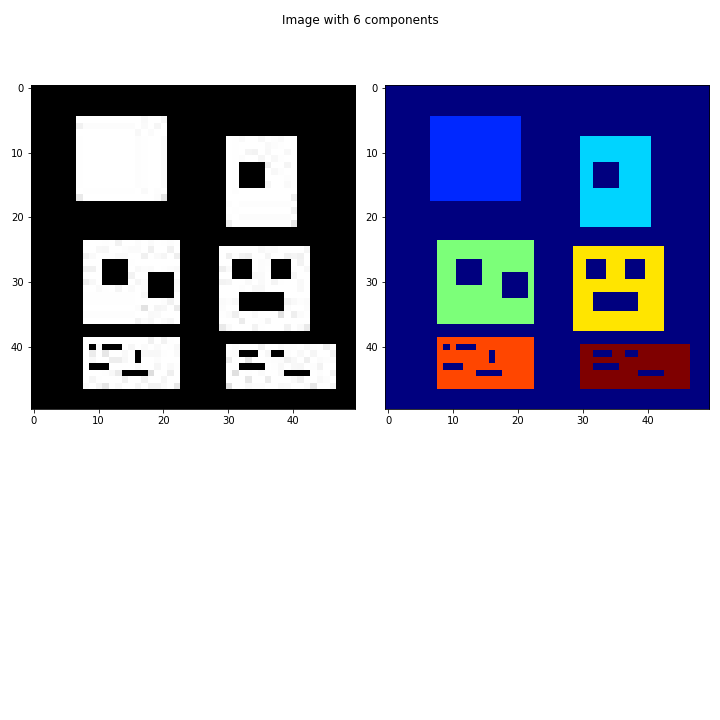
\includegraphics[width=7cm]{Figures/fig4.png}}
		\label{fig: ccl_fig4}
		\vspace{-2.0cm}
		\centerline{Fig4 após passar pelo processo de rotulação de componentes}\medskip	
	\end{minipage}
\end{figure}

\begin{figure}[!ht]
	\begin{minipage}[b]{1.0\linewidth}
		\centering
		\centerline{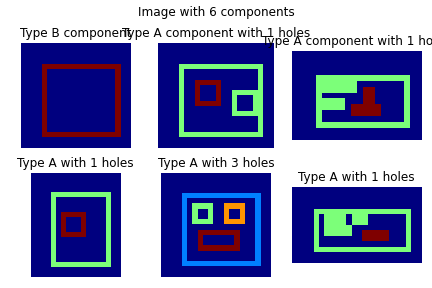
\includegraphics[width=7cm]{Figures/ccl_fig4.png}}
		\label{fig: hole_fig4}
		%\vspace{-2.0cm}
		\centerline{Fig1 após passar pelo processo de detecção de buracos}\medskip	
	\end{minipage}
\end{figure}
% -----------------------------------------------------------------
%\vfill
%\pagebreak
\newpage
\onecolumn
\section{Códigos}

\subsection{Imports}
\label{cod:imports}
\begin{python}
	import numpy as np
	import matplotlib.pyplot as plt
	import cv2
	import json
\end{python}

\subsection{bin\_ccl}
\label{cod:ccl}
\begin{python}
def image_invert(image, Bin = False):
	if(Bin):
		image[image == image.max()] = 255
	return abs(np.subtract(255, image))

def image_binarization(image, threshold = 1, 	background = 0, Bin = False):  
	if(len(image.shape) > 2):
		image = cv2.cvtColor(image, cv2.COLOR_BGR2GRAY)
	
	if(background == 1):
		image = image_invert(image, Bin = Bin)
	
	new_image = np.where(image > threshold, 1, image)
	new_image = np.where(image <= threshold, 0, image)
	
	return new_image.astype(np.uint8)

def neighbor_evaluate(image, row, col, neighborhood = 8):
	# using 8-neighborhood as default
	image_shape = image.shape
	neighbor = np.array([])
	
	if(row > 0):
		neighbor = np.concatenate([neighbor, [image[row - 1, col]]])     
	if(col > 0):
		neighbor = np.concatenate([neighbor, [image[row, col - 1]]])
	
	# To be used considering an 8-neighborhood
	if(neighborhood == 8):
		if(row > 0 and col < (image_shape[1] - 1)):
			neighbor = np.concatenate([neighbor, [image[row - 1, col + 1]]])        
		if(col > 0 and row > 0): 
			neighbor = np.concatenate([neighbor, [image[row - 1, col - 1]]])
	if(sum(neighbor) == 0):
		return 0, None # Show that there is not any neighbor greater than zero.
	
	labels = np.unique(neighbor[neighbor > 0])
	if(labels.max() != labels.min()):
		return labels.min(), {labels.max(): labels.min()}
	else:
		return labels.min(), None


def bin_ccl(image, neighborhood = 8, background = 0, threshold = 0, filtering = True,
plot = True, top_space = 1.3, color_map = 'jet', figsize = [10, 10], figname = 'fig'):
	components = 0
	label = 0
	is_one = False
	image = np.array(image)
	
	if(len(image.shape) > 2):
		image = cv2.cvtColor(image, cv2.COLOR_BGR2GRAY)
	n_rows, n_columns = image.shape
	
	if(filtering):
		image = image_binarization(image, background = background, threshold = threshold)
	
	label_image = np.copy(image)
	
	image_dict = {}
	conflict = None
	
	for i in range(n_rows):
		for j in range(n_columns):
			if(image[i][j] != 0):
				label, conflict = neighbor_evaluate(label_image, i, j, neighborhood = neighborhood)
				if(conflict is not None):
					for old, new in conflict.items():
						image_dict[old] = new
				if(not is_one):
					if(label == 0):
						components += 1
						label = components
					is_one = True
			else:
				label = 0
				is_one = False
			label_image[i][j] = label
		is_one = False
	for old, new in image_dict.items():
		label_image = np.where(label_image==old, new, label_image)
	comp_values = np.unique(label_image[label_image > 0])
	n_components = len(comp_values)

	if(plot):
		plt.figure()
		fig, axs = plt.subplots(1, 2, figsize = figsize)
		axs[0].imshow(image, cmap = 'gray', vmin = image.min(), vmax = image.max())
		axs[1].imshow(label_image, cmap = color_map, vmin = label_image.min(), vmax = label_image.max())
		fig.suptitle('Image with %d components' % n_components)
		fig.tight_layout()
		fig.subplots_adjust(top = top_space)
		plt.savefig('images/' + figname)
		plt.show()
	#         plt.savefig('images/test1.png')
	
	return {'image': label_image, 'n_objects': n_components, 'obj_ids': comp_values}
	\end{python}
	
\newpage
\subsection{hole\_detect}
\label{cod:hole_detect}
\begin{python}
def get_components(ccl_fig, tol = 4):
	image = ccl_fig['image']
	img_shape = image.shape 
	objects = []
	
	for comp in range(ccl_fig['n_objects']):
		obj =  np.zeros(img_shape)
		for i in range(img_shape[0]):
			for j in range(img_shape[1]):
				if(image[i][j] == ccl_fig['obj_ids'][comp]):
					obj[i][j] = image[i][j]
			
		x_lim = [img_shape[0], 0]
		y_lim = [img_shape[1], 0]
		
		for i in range(img_shape[0]):
			for j in range(img_shape[1]):
				if(obj[i][j] != 0):
					if(i < x_lim[0]):
						x_lim[0] = i
					elif(i > x_lim[1]):
						x_lim[1] = i
					if(j < y_lim[0]):
						y_lim[0] = j
					elif(j > y_lim[1]):
						y_lim[1] = j
						
		x_lim[0] -= tol
		y_lim[0] -= tol
		x_lim[1] += tol
		y_lim[1] += tol
		
		obj = obj[x_lim[0]: x_lim[1], y_lim[0]: y_lim[1]]
		objects.append(obj)
	return objects


def hole_detect(ccl_fig, tol = 4, gradient = True, k_data = [[0, 1, 0], [1, 1, 1], [0, 1, 0]]):
	n_outlines = []
	new_objects = []
	objects = get_components(ccl_fig)
	kernel = np.array(k_data, np.uint8)
	
	for obj in objects:
		if(gradient):
			obj = cv2.morphologyEx(obj, cv2.MORPH_GRADIENT, kernel)
		obj = image_binarization(obj, background=0, threshold = 0, Bin = True)
		fig_ccl = bin_ccl(obj, filtering = False, plot = False)
		n_outlines.append(fig_ccl['n_objects'] - 1)
		new_objects.append(fig_ccl['image'])
	return {'objects': new_objects, 'holes': n_outlines}

\end{python}

\newpage
\subsection{ccl - fig1}
\label{cod:ccl_fig1}

\begin{python}
fig1 = cv2.imread("imagens_BW/fig1.jpg")
new_fig1 = image_binarization(fig1, threshold = 100, background = 1)
ccl_fig1 = bin_ccl(new_fig1, filtering = False, neighborhood = 8, color_map = 'hot', figname = 'fig1')

figure = ccl_fig1
result = hole_detect(figure, k_data = np.ones([5, 2]))

plt.figure()
fig, axs = plt.subplots(2, int((1 + figure['n_objects'] / 2)))

for idx in range(int(np.ceil(figure['n_objects']/2))):
	axs[0][idx].imshow(result['objects'][idx*2], cmap = 'jet')
	
	if(result['holes'][idx*2] != 0):
		axs[0][idx].set_title("Type A with %d holes" % result['holes'][idx*2])
	else:
		axs[0][idx].set_title("Type B component")
	
	axs[0][idx].axis('off')
	
	if((idx*2 + 1) < figure['n_objects']):
		axs[1][idx].imshow(result['objects'][idx*2 + 1], cmap = 'jet')
		
		if(result['holes'][idx*2 + 1] != 0):
			axs[1][idx].set_title("Type A with %d holes" % result['holes'][idx*2 + 1])
		else:
			axs[1][idx].set_title("Type B")        
		
		axs[1][idx].axis('off')
	else:
		fig.delaxes(axs[1][idx])
fig.suptitle('Image with %d components' % figure['n_objects'])
fig.tight_layout()
fig.subplots_adjust(top = 0.85)
plt.savefig('images/ccl_fig1')
plt.show()	
\end{python}

\newpage
\subsection{ccl - fig2}
\label{cod:ccl_fig2}

\begin{python}
fig2 = cv2.imread("imagens_BW/fig2.jpg")
fig2 = image_binarization(fig2, background = 1, threshold = 180)

k1_data = np.ones([4, 3])
kernel1 = np.array(k1_data, np.uint8)

fig2 = cv2.morphologyEx(fig2, cv2.MORPH_CLOSE, kernel1)
ccl_fig2 = bin_ccl(fig2, neighborhood = 8, filtering = False, color_map = 'hot', figname = 'fig2')

\end{python}

\newpage
\subsection{ccl - fig3}
\label{cod:ccl_fig3}

\begin{python}
fig3 = cv2.imread("imagens_BW/fig3.jpg")
fig3 = image_binarization(fig3, background = 1, threshold = 0)

k_data = np.ones([3, 3])
kernel = np.array(k_data, np.uint8)

fig3 = cv2.morphologyEx(fig3, cv2.MORPH_CLOSE, kernel)

ccl_fig3 = bin_ccl(fig3, background = 1, neighborhood = 8, filtering = False, figname = 'fig3')
figure = ccl_fig3
result = hole_detect(figure, gradient = False, k_data = np.ones([3, 3]))

plt.figure()
fig, axs = plt.subplots(2, int((figure['n_objects'] / 2)))

for idx in range(int(np.ceil(figure['n_objects']/2))):
	axs[0].imshow(result['objects'][idx*2], cmap = 'jet')
	
	if(result['holes'][idx*2] != 0):
		axs[0].set_title("Type A with %d holes" % result['holes'][idx*2])
	else:
		axs[0].set_title("Type B")
	
	axs[0].axis('off')
	
	if((idx*2 + 1) < figure['n_objects']):
		axs[1].imshow(result['objects'][idx*2 + 1], cmap = 'jet')
		
		if(result['holes'][idx*2 + 1] != 0):
			axs[1].set_title("Type A with %d holes" % result['holes'][idx*2 + 1])
		else:
			axs[1].set_title("Type B")        
	
		axs[1].axis('off')
	else:
		fig.delaxes(axs[1][idx])
fig.suptitle('Image with %d components' % figure['n_objects'])
fig.tight_layout()
fig.subplots_adjust(top = 0.85)
plt.savefig('images/ccl_fig3')
plt.show()
\end{python}

\newpage
\subsection{ccl - fig4}
\label{cod:ccl_fig4}

\begin{python}
fig4 = cv2.imread("imagens_BW/fig4.jpg")

ccl_fig4 = bin_ccl(fig4, background = 1, neighborhood = 8, threshold = 100, figname = 'fig4')

figure = ccl_fig4
# figure = cv2.morphologyEx(figure, cv2.MORPH_OPEN, np.array(np.ones([2, 2]), np.uint8))
result = hole_detect(figure, gradient = True, k_data = np.ones([2, 2]))

plt.figure()
fig, axs = plt.subplots(2, int((figure['n_objects'] / 2)))

for idx in range(int(np.ceil(figure['n_objects']/2))):
axs[0][idx].imshow(result['objects'][idx*2], cmap = 'jet')
	
	if(result['holes'][idx*2] != 0):
		axs[0][idx].set_title("Type A component with %d holes" % result['holes'][idx*2])
	else:
		axs[0][idx].set_title("Type B component")
	
	axs[0][idx].axis('off')
	
	if((idx*2 + 1) < figure['n_objects']):
		axs[1][idx].imshow(result['objects'][idx*2 + 1], cmap = 'jet')
		
		if(result['holes'][idx*2 + 1] != 0):
			axs[1][idx].set_title("Type A with %d holes" % result['holes'][idx*2 + 1])
		else:
			axs[1][idx].set_title("Type B")        
	
		axs[1][idx].axis('off')
	else:
	f	ig.delaxes(axs[1][idx])
fig.suptitle('Image with %d components' % figure['n_objects'])
fig.tight_layout()
fig.subplots_adjust(top = 0.85)
plt.savefig('images/ccl_fig4')
plt.show()

\end{python}

\end{document}
